\section{Auswertung}
Das für die Auswertung der angefertigten Bilder und der Bestimmung der Interferenzmaxima verwendete Programm ist das Paket \textit{Fiji} der open-source-Anwendung \textit{ImageJ} \cite{Fiji}.

\subsection{Eichung des Magnetfeldes}
Zu Beginn des Auswertung soll das Magnetfeld des Elektromagneten geeicht werden. Hierzu werden die Strom-Magnetfeld-Paare für das ansteigende und das abfallende Magnetfeld aus Tabelle \ref{tab:eichen} grafisch aufgetragen.
Durch eine lineare Ausgleichsrechnung der Form
\begin{equation}
  B(I)=aI+b
\end{equation}
soll ein möglichst exaktes Bestimmen des über den Strom $I$ eingestellen Magnetfeldes $B$ erreicht werden.
Zu sehen ist dieser Zusammenhang in Abbildung \ref{abb:eichung}.
Als Parameter der Ausgleichsrechnung ergeben sich
\begin{align*}
  a &= \SI{183,3 \pm 7,9}{\milli\tesla\per\ampere},\\
    b &= \SI{-36,0 \pm 27,8}{\milli\tesla}\;.
\end{align*}

Insgesamt lassen sich somit die Magnetfelder für die im Experiment eingestellten Ströme zu \ref{tab:Bfelder} berechnen:
\begin{table}[H]
  \centering
  \caption{Aus der linearen Ausgeichsrechnung bestimmte Magnetfelder $B$ für die im Experiment angelegten Ströme $I$.}
  \label{tab:Bfelder}
  \begin{tabular}{cc}
    \toprule
    {$I \:/\: \si{\ampere}$} & {$B \:/\: \si{\milli\tesla}$}\\
    \midrule
  2,5 & 422 \pm 34 \\
  3,8 & 660 \pm 40 \\
  6,0 & 1060 \pm 50
  \end{tabular}
\end{table}
\clearpage
\begin{table}[H]
  \centering
  \caption{Messwerte der Magnetfeldstärke $B$ in Abhängigkeit der Stromstärke $I$ des verwendeten Elektromagneten jeweils bei ansteigenden und abfallenden Feldern.}
  \label{tab:eichen}
  \begin{tabular}{c|cc}
    \toprule
    {$I \:/\: \si{\ampere}$} & {$B_\text{steigend} \:/\: \si{\milli\tesla}$} & {$B_\text{fallend} \:/\: \si{\milli\tesla}$} \\
    \midrule
  0.0    &     5,5  &    6,3  \\
  0.5    &    111,8  &   105,3  \\
  1.0    &   155,5  &  163,7  \\
  1.5    &   242,4  &  244,1  \\
  2.0    &   318,2  &  310,3  \\
  2.5    &   390,0  &  406,9  \\
  3.0    &   469,9  &  474,7  \\
  3.5    &   550,7  &  554,9  \\
  4.0    &   629,2  &  642,8  \\
  4.5    &   734,7  &  746,6  \\
  5.0    &   880,9  &  879,2  \\
  5.5    &   1042,0  &  1015,4  \\
  6.0    &   1150,5  &  1150,5  \\
  \end{tabular}
\end{table}

\begin{figure}
  \centering
  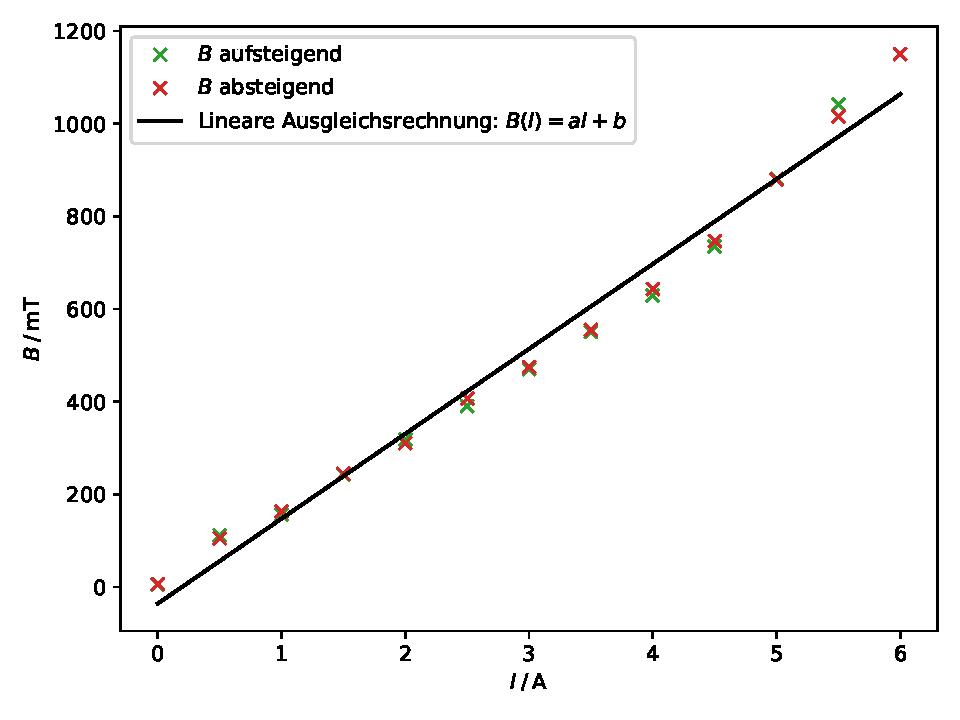
\includegraphics[width=0.7\textwidth]{plots/eichung.pdf}
  \caption{Das mit einer Hall-Sonde gemessene Magnetfeld $B$ in Abhängigkeit des eingestellten Stroms $I$ für ein Auf- und ein Absteigen. Ebenso eine lineare Ausgleichsrechnung zur Bestimmung des Wertepaarzusammenhangs.}
  \label{abb:eichung}
\end{figure}
\clearpage
\subsection{Messung des Landé-Faktors}
Im Folgenden sollen nun die Breiten der Interferenzstreifen ohne angelegtes Magnetfeld $\deltaup$ und unter Einfluss eines angelegten Magnetfeldes $\Deltaup$ bestimmt werden.
Für die Wellenlängendifferenzen ergibt sich unter Verwendung der in Abschnitt \ref{sec:dispersion} bestimmten $\Deltaup \lambda$:
\begin{equation}
  \deltaup \lambda = \frac{1}{2}\frac{\deltaup s}{\Deltaup s}\Deltaup \lambda\,.
  \label{eq:difflambda}
\end{equation}
Die Energiedifferenz aufgrund eines angelegten Magnetfeldes ergibt sich zu
\begin{equation}
  |\Deltaup E| = |\Deltaup m| g \mu_B B\,.
\end{equation}
Für die Energie lässt sich $E=\frac{\hbar c}{\lambda}$ einsetzen und nach $\lambda$ ableiten.
Über Umformen des für $\deltaup \lambda$ eingesetzten Zusammenhangs \eqref{eq:difflambda} nach dem Landé-Faktor ergibt sich für die erlaubten Übergänge mit $|\Deltaup m|=1$
\begin{equation}
  g=\frac{\hbar c \deltaup \lambda}{\lambda^2 \mu_B B}\,.
  \label{eq:g}
\end{equation}
Mittels des Pakets \textit{Fiji} werden nun die aufgenommenen Fotographien auf ihren Farbkontrast hin ausgewertet.
Hierüber lassen sich die Abstände $\Deltaup$ und $\deltaup$ bestimmen.
Bei der Aufnahme der Bilder ist mit einem konstanten Zoom von \textit{30x} gearbeitet worden, sodass ein Herausrechnen nicht nötig ist.
\subsection{Vermessung der \texorpdfstring{$\sigma$}{sigma}-Komponente der roten Linie}
Zu Beginn werden die erhaltenen Maxima aus Tabelle \ref{tab:sigmarot660mT} gezählt und mithilfe der Abstände auf einen gemittelten Abstand von
\begin{equation}
\deltaup s= \SI{59,05}{px}
\end{equation}
heruntergerechnet. Da bei der Versuchsdurchführung kein Bild von dieser Polarisation ohne Magnetfeld aufgenommen wurde, muss hier eine weitere Auswertung entfallen.

\begin{table}[H]
  \centering
  \caption{Mit dem Programm \textit{Fiji} \cite{Fiji} ausgelesene Intensitätsmaxima zur Bestimmung der Abstände $\deltaup s$ für die rote Spektrallinie mit einem angelegten Magnetfeld $B=\SI{660 \pm 40}{\milli\tesla}$  unter einem Polarisationswinkel von $0°$.}
  \label{tab:sigmarot660mT}
  \begin{tabular}{c|cc}
    \toprule
    {Nummer} & {$x \:/\: \si{px}$} & {$y \:/\: \text{bel. Einheiten}$}\\
    \midrule
 1 &   59  &	 26,26 \\
 2 &   94  &	 26,67 \\
 3 &  162  &	 28,25 \\
 4 &  233  &	 29,17 \\
 5 &  294  &	 30,53 \\
 6 &  366  &	 31,15 \\
 7 &  426  &	 32,12 \\
 8 &  491  &	 33,44 \\
 9 &  551  &  33,45 \\
10 &  615  &	 32,98 \\
11 &  673  &	 34,43 \\
12 &  735  &	 34,33 \\
13 &  791  &	 35,11 \\
14 &  850  &	 34,92 \\
15 &  903  &	 34,16 \\
16 &  964  &	 33,92 \\
17 & 1014  &	 34,41 \\
18 & 1073  &	 33,10 \\
19 & 1122  &	 31,97 \\
  \end{tabular}
\end{table}
\begin{figure}
  \centering
  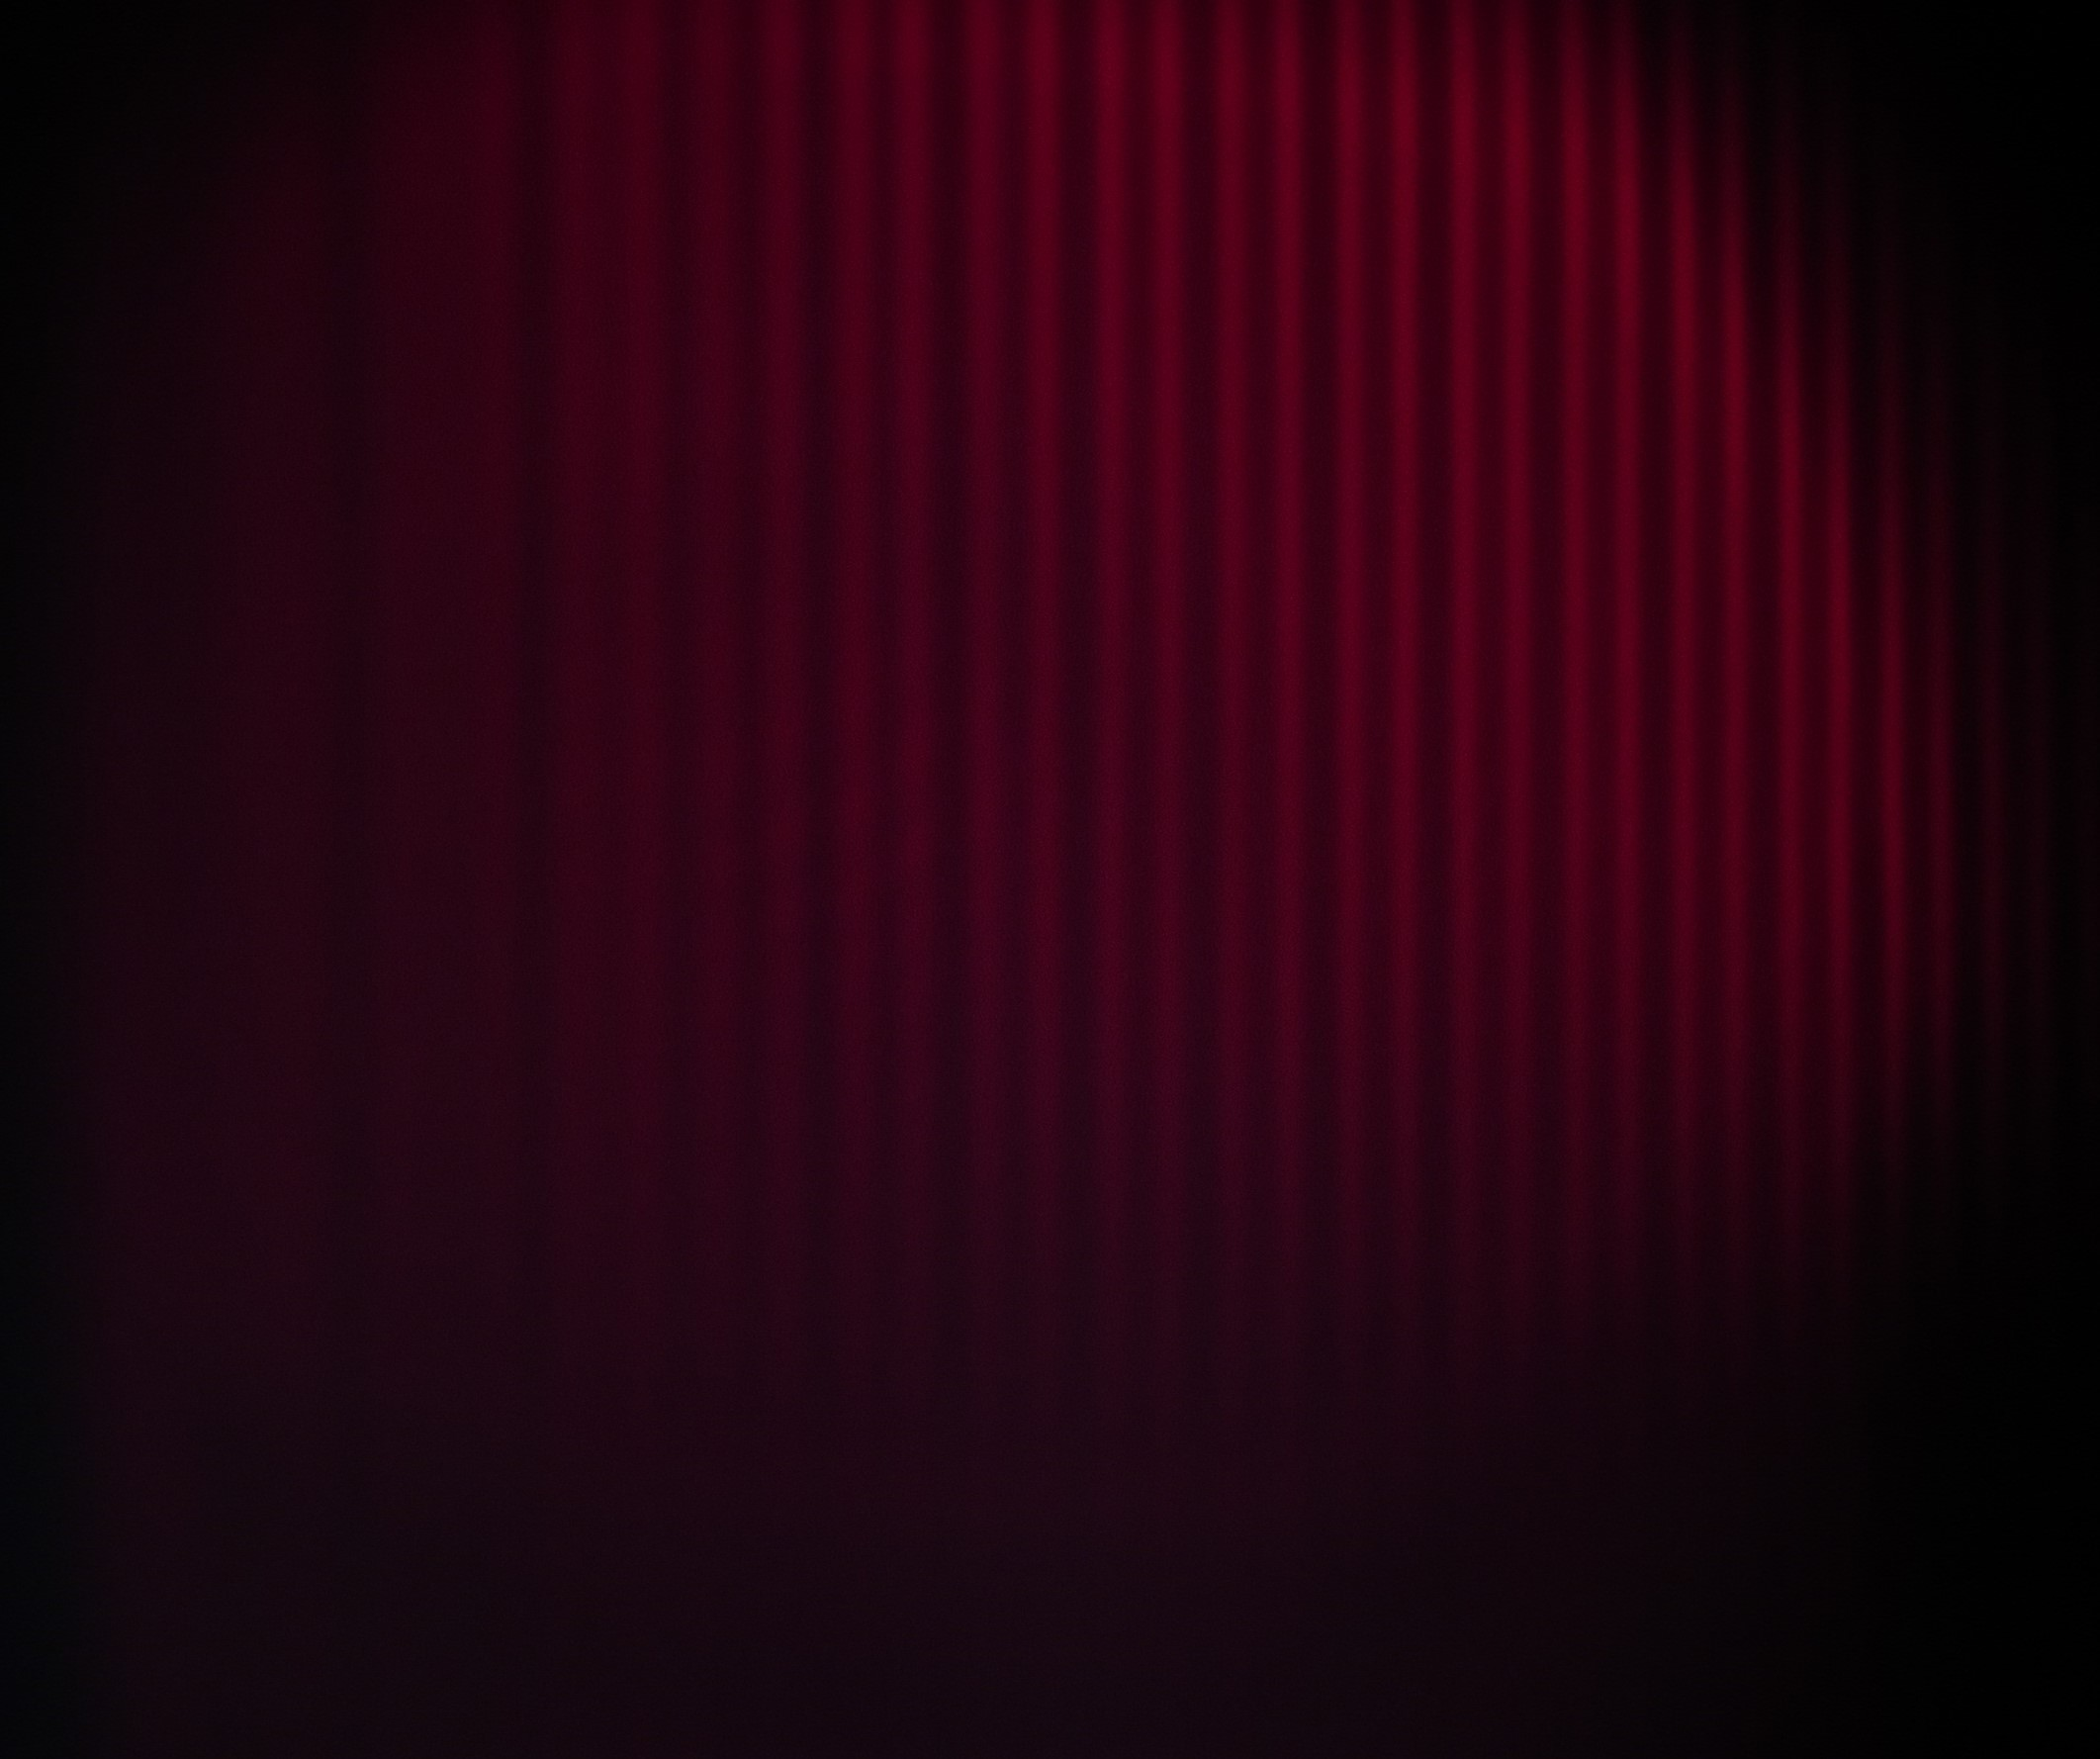
\includegraphics[width=0.5\textwidth]{bilder/2995_ROT_621mT_sigma.jpg}
  \caption{Fotographie der Interferenzlinien der Lummer-Gehrcke-Platte für die $\sigma$-Linie des roten Lichts bei einem angelegten Magnetfeld von $B=\SI{660 \pm 40}{\milli\tesla}$.}
  \label{abb:sigmarot660mT}
\end{figure}
\begin{figure}
  \centering
  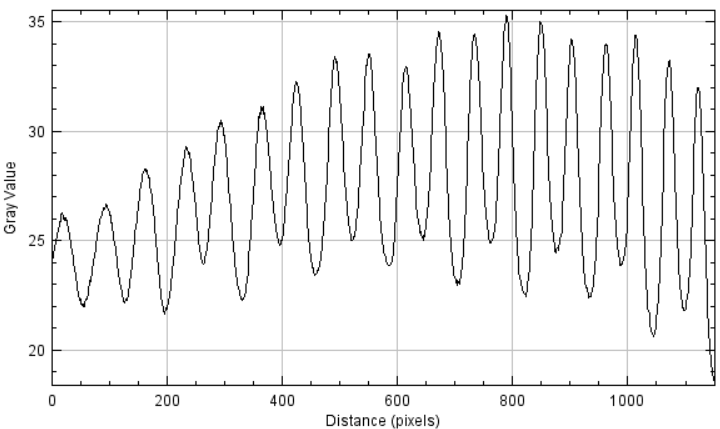
\includegraphics[width=0.7\textwidth]{bilder/sigmaROT_620mT.PNG}
  \caption{Kontrastauswertung der Interferenzintensität für die $\sigma$-Linie des roten Lichts bei einem angelegten Magnetfeld von $B=\SI{660 \pm 40}{\milli\tesla}$. Aufgetragen ist die Intensität in beliebigen Einheiten gegen den Abstand in $x$-Richtung in Einheiten von Pixeln.}
  \label{abb:plotsigmarot660mT}
\end{figure}

\subsection{Vermessung der \texorpdfstring{$\sigma$}{sigma}-Komponente der blauen Linie}
Für die $\sigma$-Komponente sind Bilder mit und ohne Magnetfeld aufgenommen worden, sodass hier eine komplette Auswertung vorgenommen werden kann. Betrachtet man Tabelle \ref{tab:sigmablau0mT}, so lässt sich ein mittlerer Abstand von
\begin{equation}
  \Deltaup s=\SI{104,5}{px}
\end{equation}
bestimmen. Die zugeschnittene Bildaufnahme ist in Abbildung \ref{abb:sigmablau0mT} zu sehen; der Grayscale-Auswertungsplot zur Bestimmung der Intensitätsmaxima in Abbildung \ref{abb:plotsigmablau0mT}.\\
Nach Zuschalten eines Magnetfeldes von $B=\SI{422\pm34}{\milli\tesla}$ ergeben sich folgende Abbildungen \ref{abb:sigmablau0mT} und \ref{abb:plotsigmablau0mT}. Mithilfe von Tabelle \ref{tab:sigmablau422mT} kann ein gemittelter Maximaabstand von
\begin{equation}
\deltaup s=\SI{99,9}{px}
\end{equation}
ermittelt werden.
Über die Formeln \eqref{eq:difflambda} und \eqref{eq:g} lässt sich ein g-Faktor für die blaue $\sigma$-Linie von
\begin{equation}
 g_{\text{blau},\sigma}=2,94
\end{equation}
bestimmt werden. Dem Vergleich mit dem Theoriewert, der sich als Mittelwert von 1,5 und 2,0 zu $g_{\text{blau},\sigma,\text{theo}}=1,75$ ergibt, folgt eine Abweichung von $\SI{68}{\%}$.

\begin{table}[H]
  \centering
  \caption{Mit dem Programm \textit{Fiji} \cite{Fiji} ausgelesene Intensitätsmaxima zur Bestimmung der Abstände $\Deltaup s$ für die blaue Spektrallinie ohne angelegtes Magnetfeld unter einem Polarisationswinkel von $0°$.}
  \label{tab:sigmablau0mT}
  \begin{tabular}{c|cc}
    \toprule
    {Nummer} & {$x \:/\: \si{px}$} & {$y \:/\: \text{bel. Einheiten}$}\\
    \midrule
 1 &   30  &	 24,68 \\
 2 &   159  &	 32,23 \\
 3 &  279  &	 38,19 \\
 4 &  385  &	 43,61 \\
 5 &  495  &	 46,26 \\
 6 &  596  &	 48,02 \\
 7 &  697  &	 48,52 \\
 8 &  792  &	 49,89 \\
 9 &  890  &   48,70 \\
10 &  983  &	 47,78 \\
11 &  1075  &	 45,08 \\
  \end{tabular}
\end{table}

\begin{figure}
  \centering
  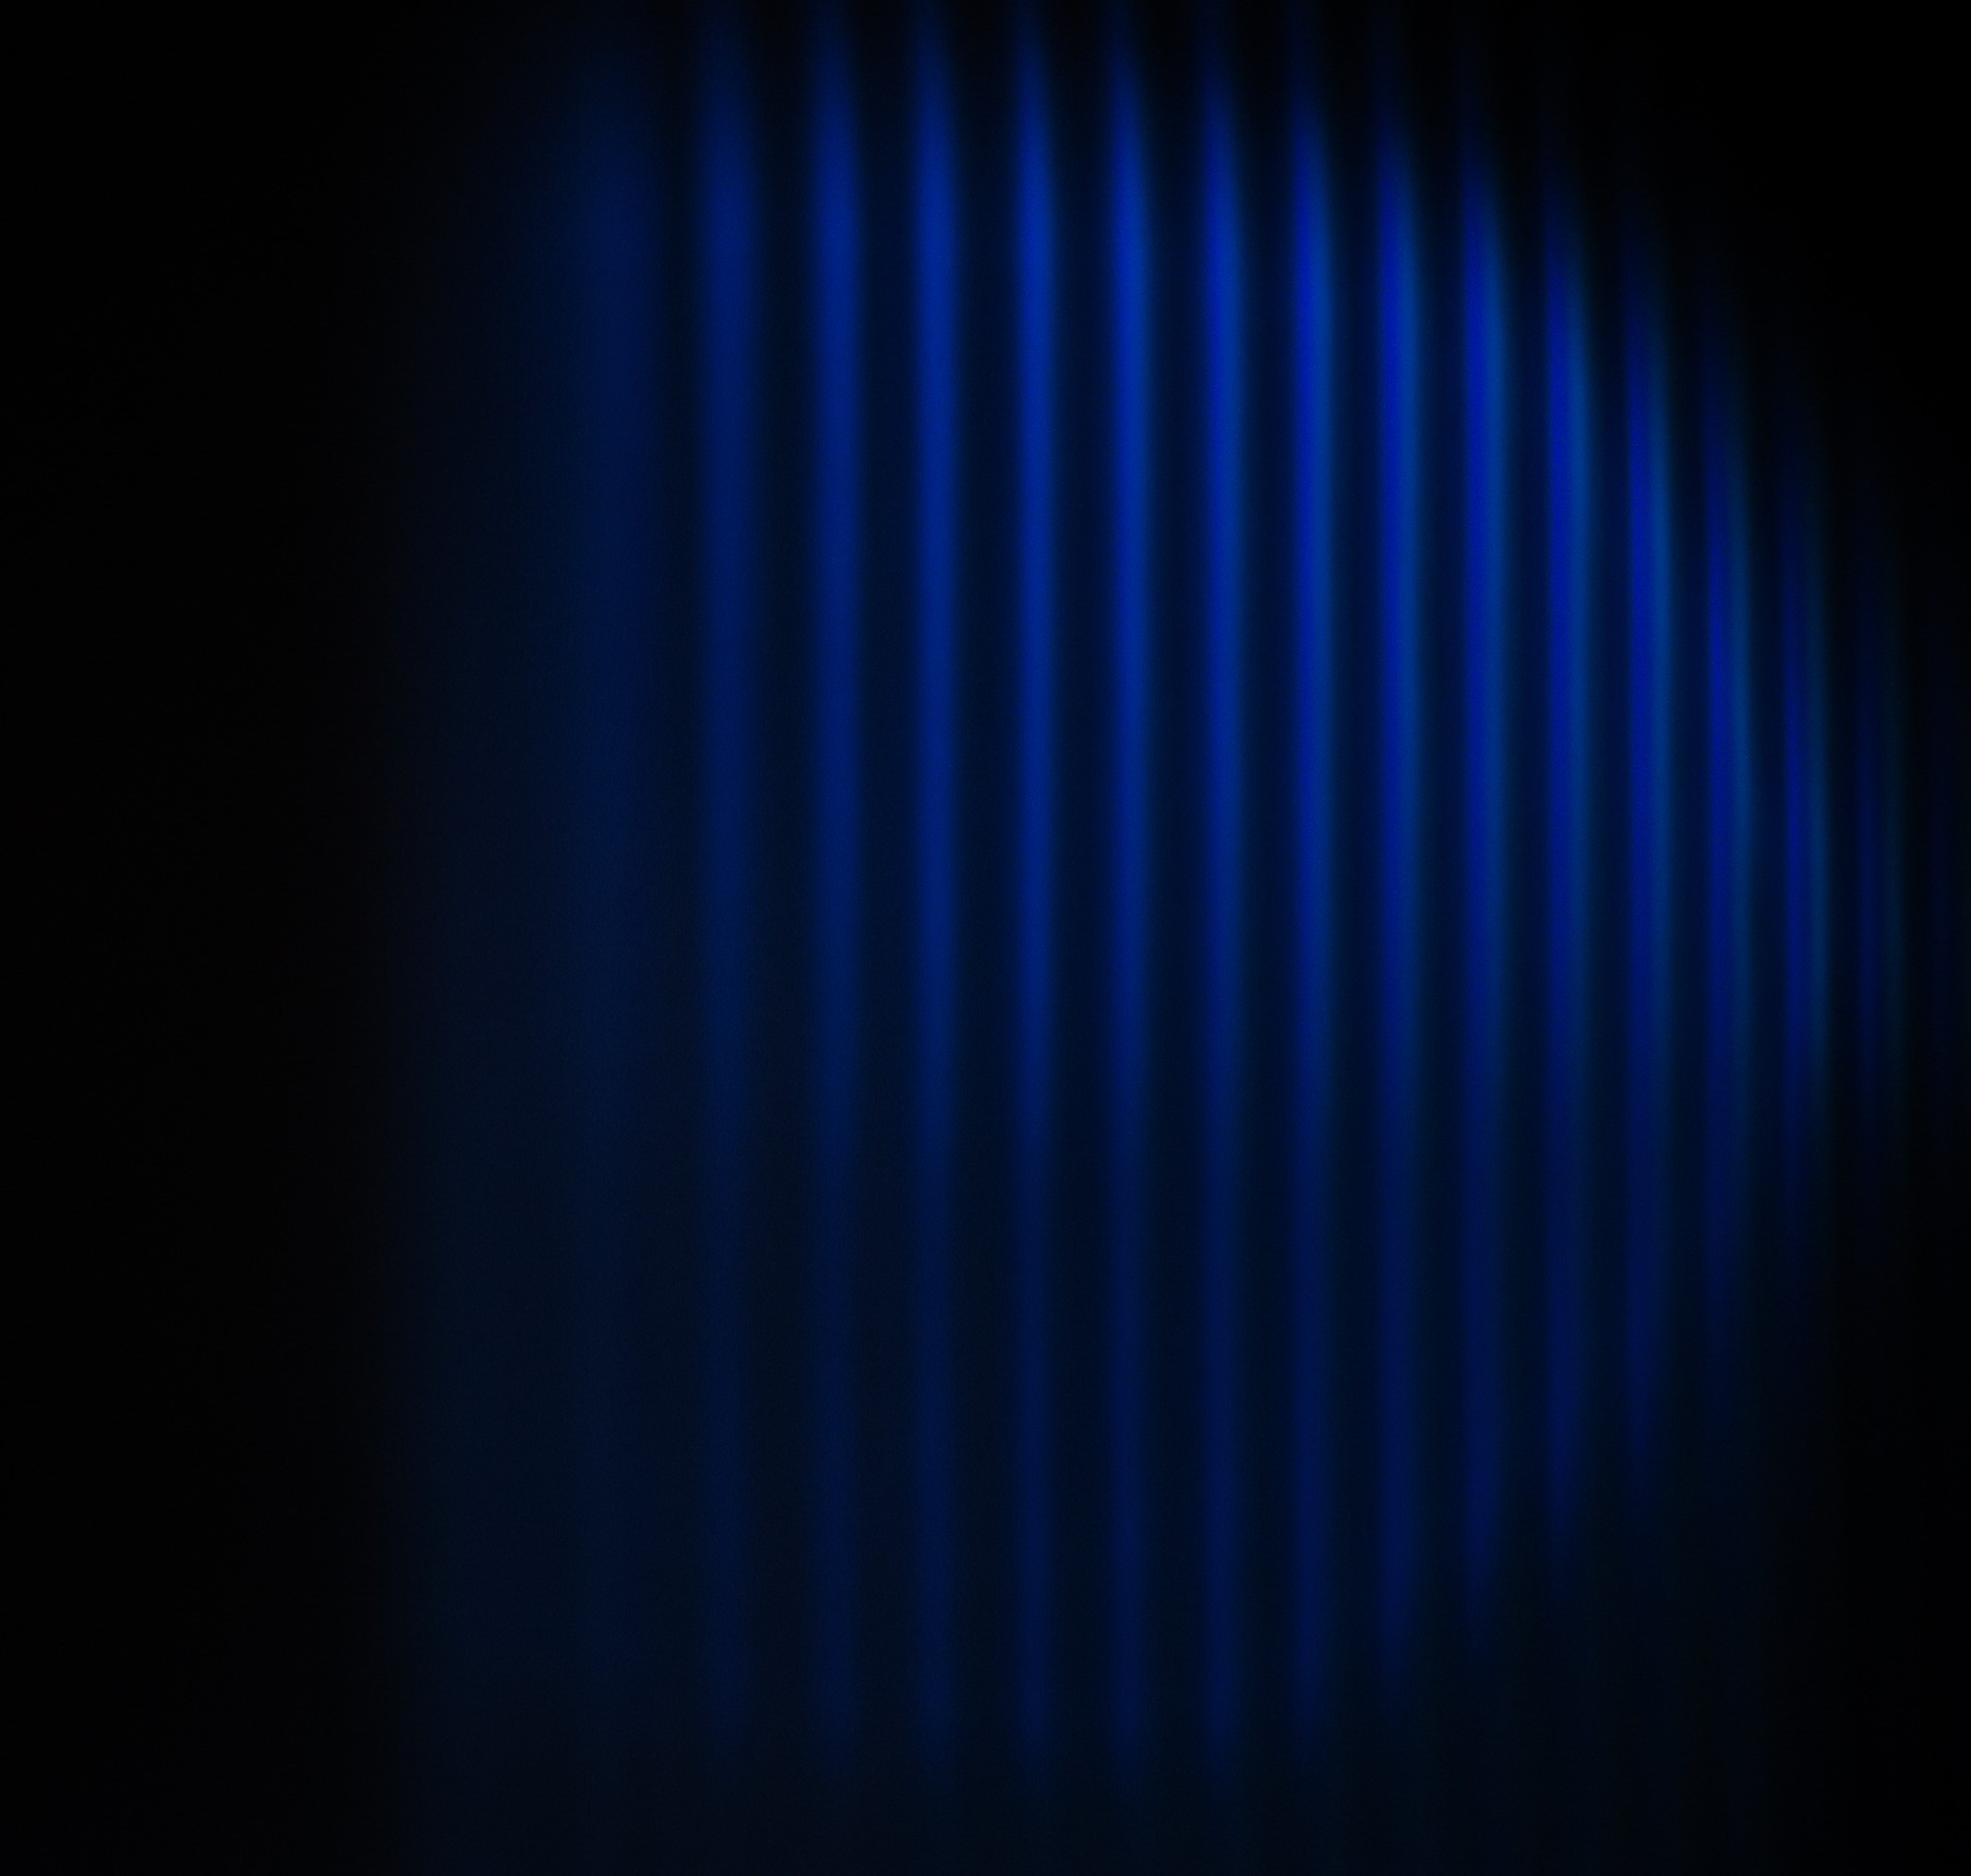
\includegraphics[width=0.5\textwidth]{bilder/3000_BLAU_0mT_sigma.jpg}
  \caption{Fotographie der Interferenzlinien der Lummer-Gehrcke-Platte für die $\sigma$-Linie des blauen Lichts ohne ein angelegtes Magnetfeld.}
  \label{abb:sigmablau0mT}
\end{figure}
\begin{figure}
  \centering
  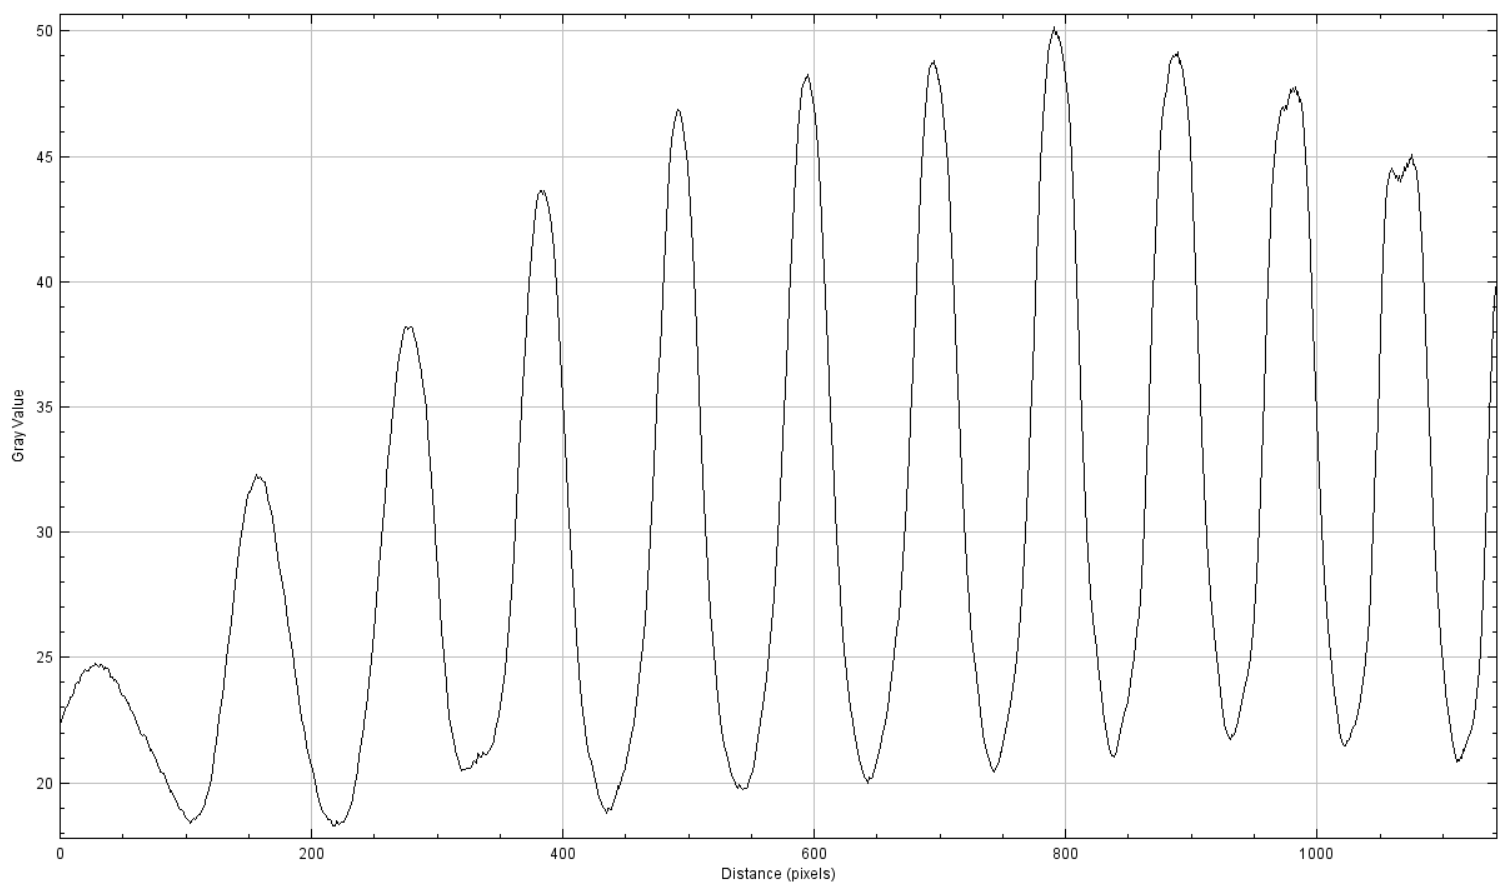
\includegraphics[width=0.7\textwidth]{bilder/sigmaBLAU_0mT.PNG}
  \caption{Kontrastauswertung der Interferenzintensität für die $\sigma$-Linie des blauen Lichts ohne angelegtes Magnetfeld. Aufgetragen ist die Intensität in beliebigen Einheiten gegen den Abstand in $x$-Richtung in Einheiten von Pixeln.}
  \label{abb:plotsigmablau0mT}
\end{figure}
%---------------------------------------------------------------------------------------------
\begin{table}[H]
  \centering
  \caption{Mit dem Programm \textit{Fiji} \cite{Fiji} ausgelesene Intensitätsmaxima zur Bestimmung der Abstände $\deltaup s$ für die blaue Spektrallinie mit einem angelegten Magnetfeld $B=\SI{422\pm34}{\milli\tesla}$  unter einem Polarisationswinkel von $0°$.}
  \label{tab:sigmablau422mT}
  \begin{tabular}{c|cc}
    \toprule
    {Nummer} & {$x \:/\: \si{px}$} & {$y \:/\: \text{bel. Einheiten}$}\\
    \midrule
 1 &  282  &	 50,83 \\
 2 &  398  &	 58,45 \\
 3 &  497  &	 60,53 \\
 4 &  604  &	 63,20 \\
 5 &  703  &	 63,85 \\
 6 &  801  &	 65,75 \\
 7 &  902  &	 67,11 \\
 8 &  996  &	 66,50 \\
 9 &  1088 &   66,26 \\
10 &  1181 &	 66,03 \\
  \end{tabular}
\end{table}

\begin{figure}
  \centering
  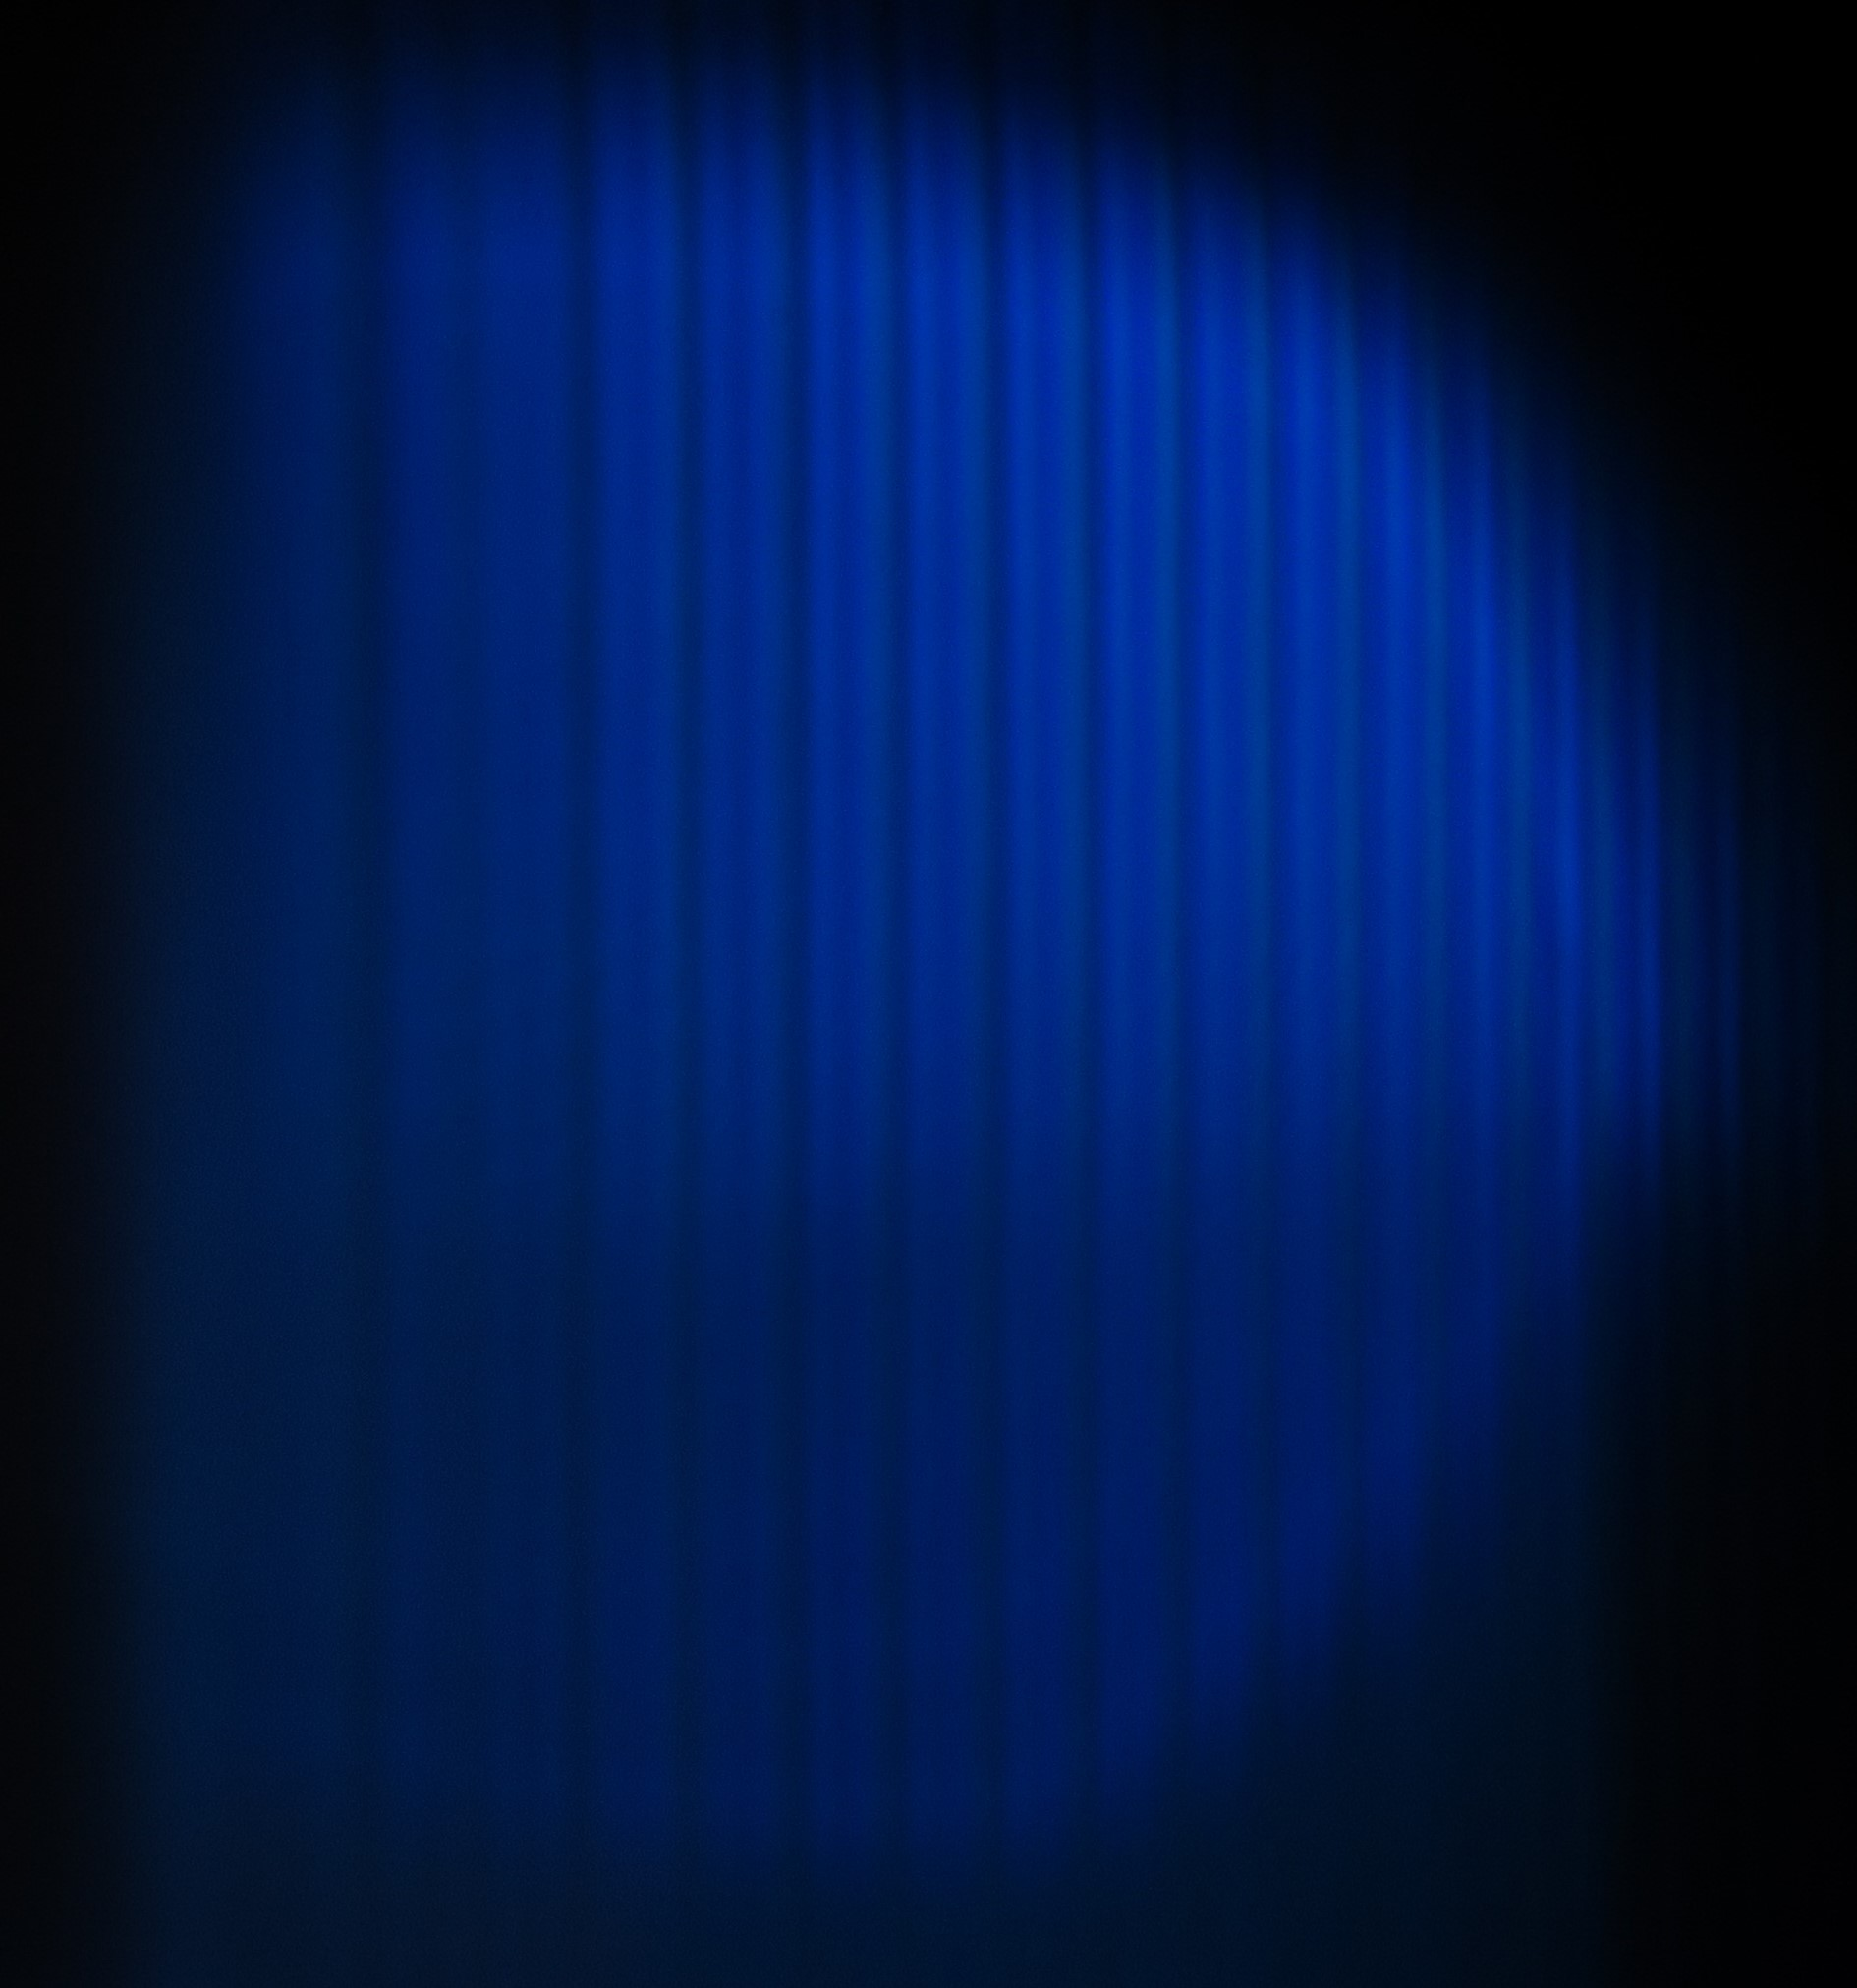
\includegraphics[width=0.5\textwidth]{bilder/3003_BLAU_300mT_sigma.jpg}
  \caption{Fotographie der Interferenzlinien der Lummer-Gehrcke-Platte für die $\sigma$-Linie des blauen Lichts bei einem angelegten Magnetfeld von $B=\SI{422\pm34}{\milli\tesla}$.}
  \label{abb:sigmablau422mT}
\end{figure}
\begin{figure}
  \centering
  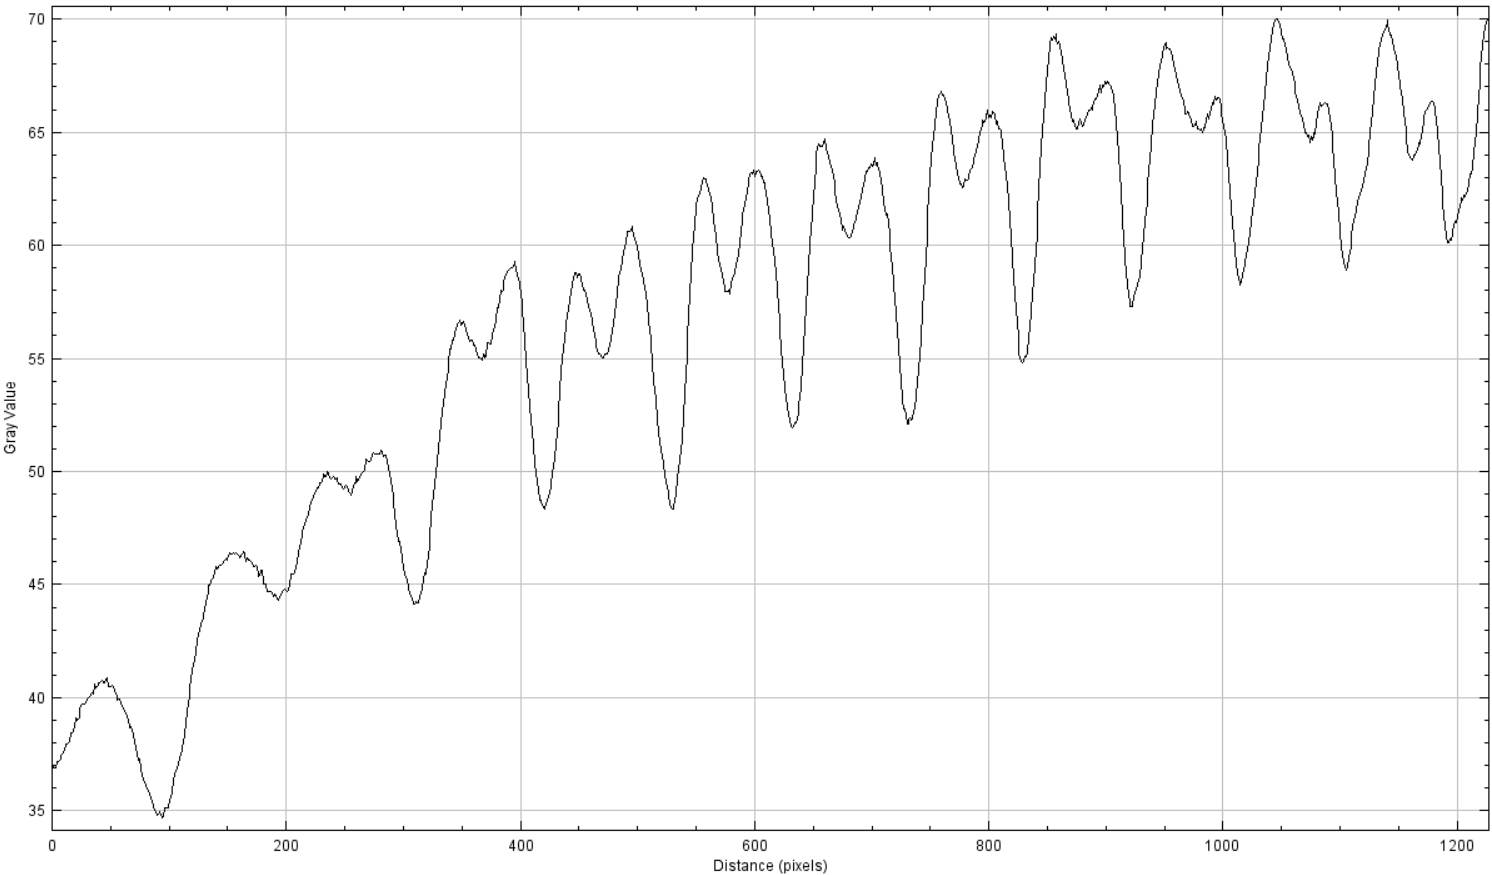
\includegraphics[width=0.7\textwidth]{bilder/sigmaBLAU_300mT.PNG}
  \caption{Kontrastauswertung der Interferenzintensität für die $\sigma$-Linie des blauen Lichts bei einem angelegten Magnetfeld von $B=\SI{422\pm34}{\milli\tesla}$. Aufgetragen ist die Intensität in beliebigen Einheiten gegen den Abstand in $x$-Richtung in Einheiten von Pixeln.}
  \label{abb:plotsigmablau422mT}
\end{figure}
\clearpage
\subsection{Vermessung der \texorpdfstring{$\pi$}{pi}-Komponente der blauen Linie}
Gleiches Vorgehen folgt ebenso für die $\pii$-Komponente der blauen Linie.
Es folgen
\begin{equation}
  \Deltaup s=\SI{100,8}{px}
\end{equation}
und
\begin{equation}
  \deltaup s=\SI{83,29}{px}\,.
\end{equation}
Folgend ist ein g-Faktor von
\begin{equation}
  g_{\text{blau},\pii}=1,01
\end{equation}
und eine Abweichung von $\SI{50}{\%}$ von dem Theoriewert von $g_{\text{blau},\sigma,\text{theo}}=0,5$.
\begin{table}[H]
  \centering
  \caption{Mit dem Programm \textit{Fiji} \cite{Fiji} ausgelesene Intensitätsmaxima zur Bestimmung der Abstände $\Deltaup s$ für die blaue Spektrallinie ohne angelegtes Magnetfeld unter einem Polarisationswinkel von $90°$.}
  \label{tab:piblau0mT}
  \begin{tabular}{c|cc}
    \toprule
    {Nummer} & {$x \:/\: \si{px}$} & {$y \:/\: \text{bel. Einheiten}$}\\
    \midrule
 1 &  32   &	 50,38 \\
 2 &  152  &	 56,97 \\
 3 &  260  &	 61,86 \\
 4 &  365  &	 65,09 \\
 5 &  469  &	 65,66 \\
 6 &  567  &	 65,99 \\
 7 &  667  &	 66,51 \\
 8 &  760  &	 65,53\\
 9 &  859  &   64,31 \\
10 &  948  &	 62,67 \\
11 &  1040  &	 62,72 \\
  \end{tabular}
\end{table}

\begin{figure}
  \centering
  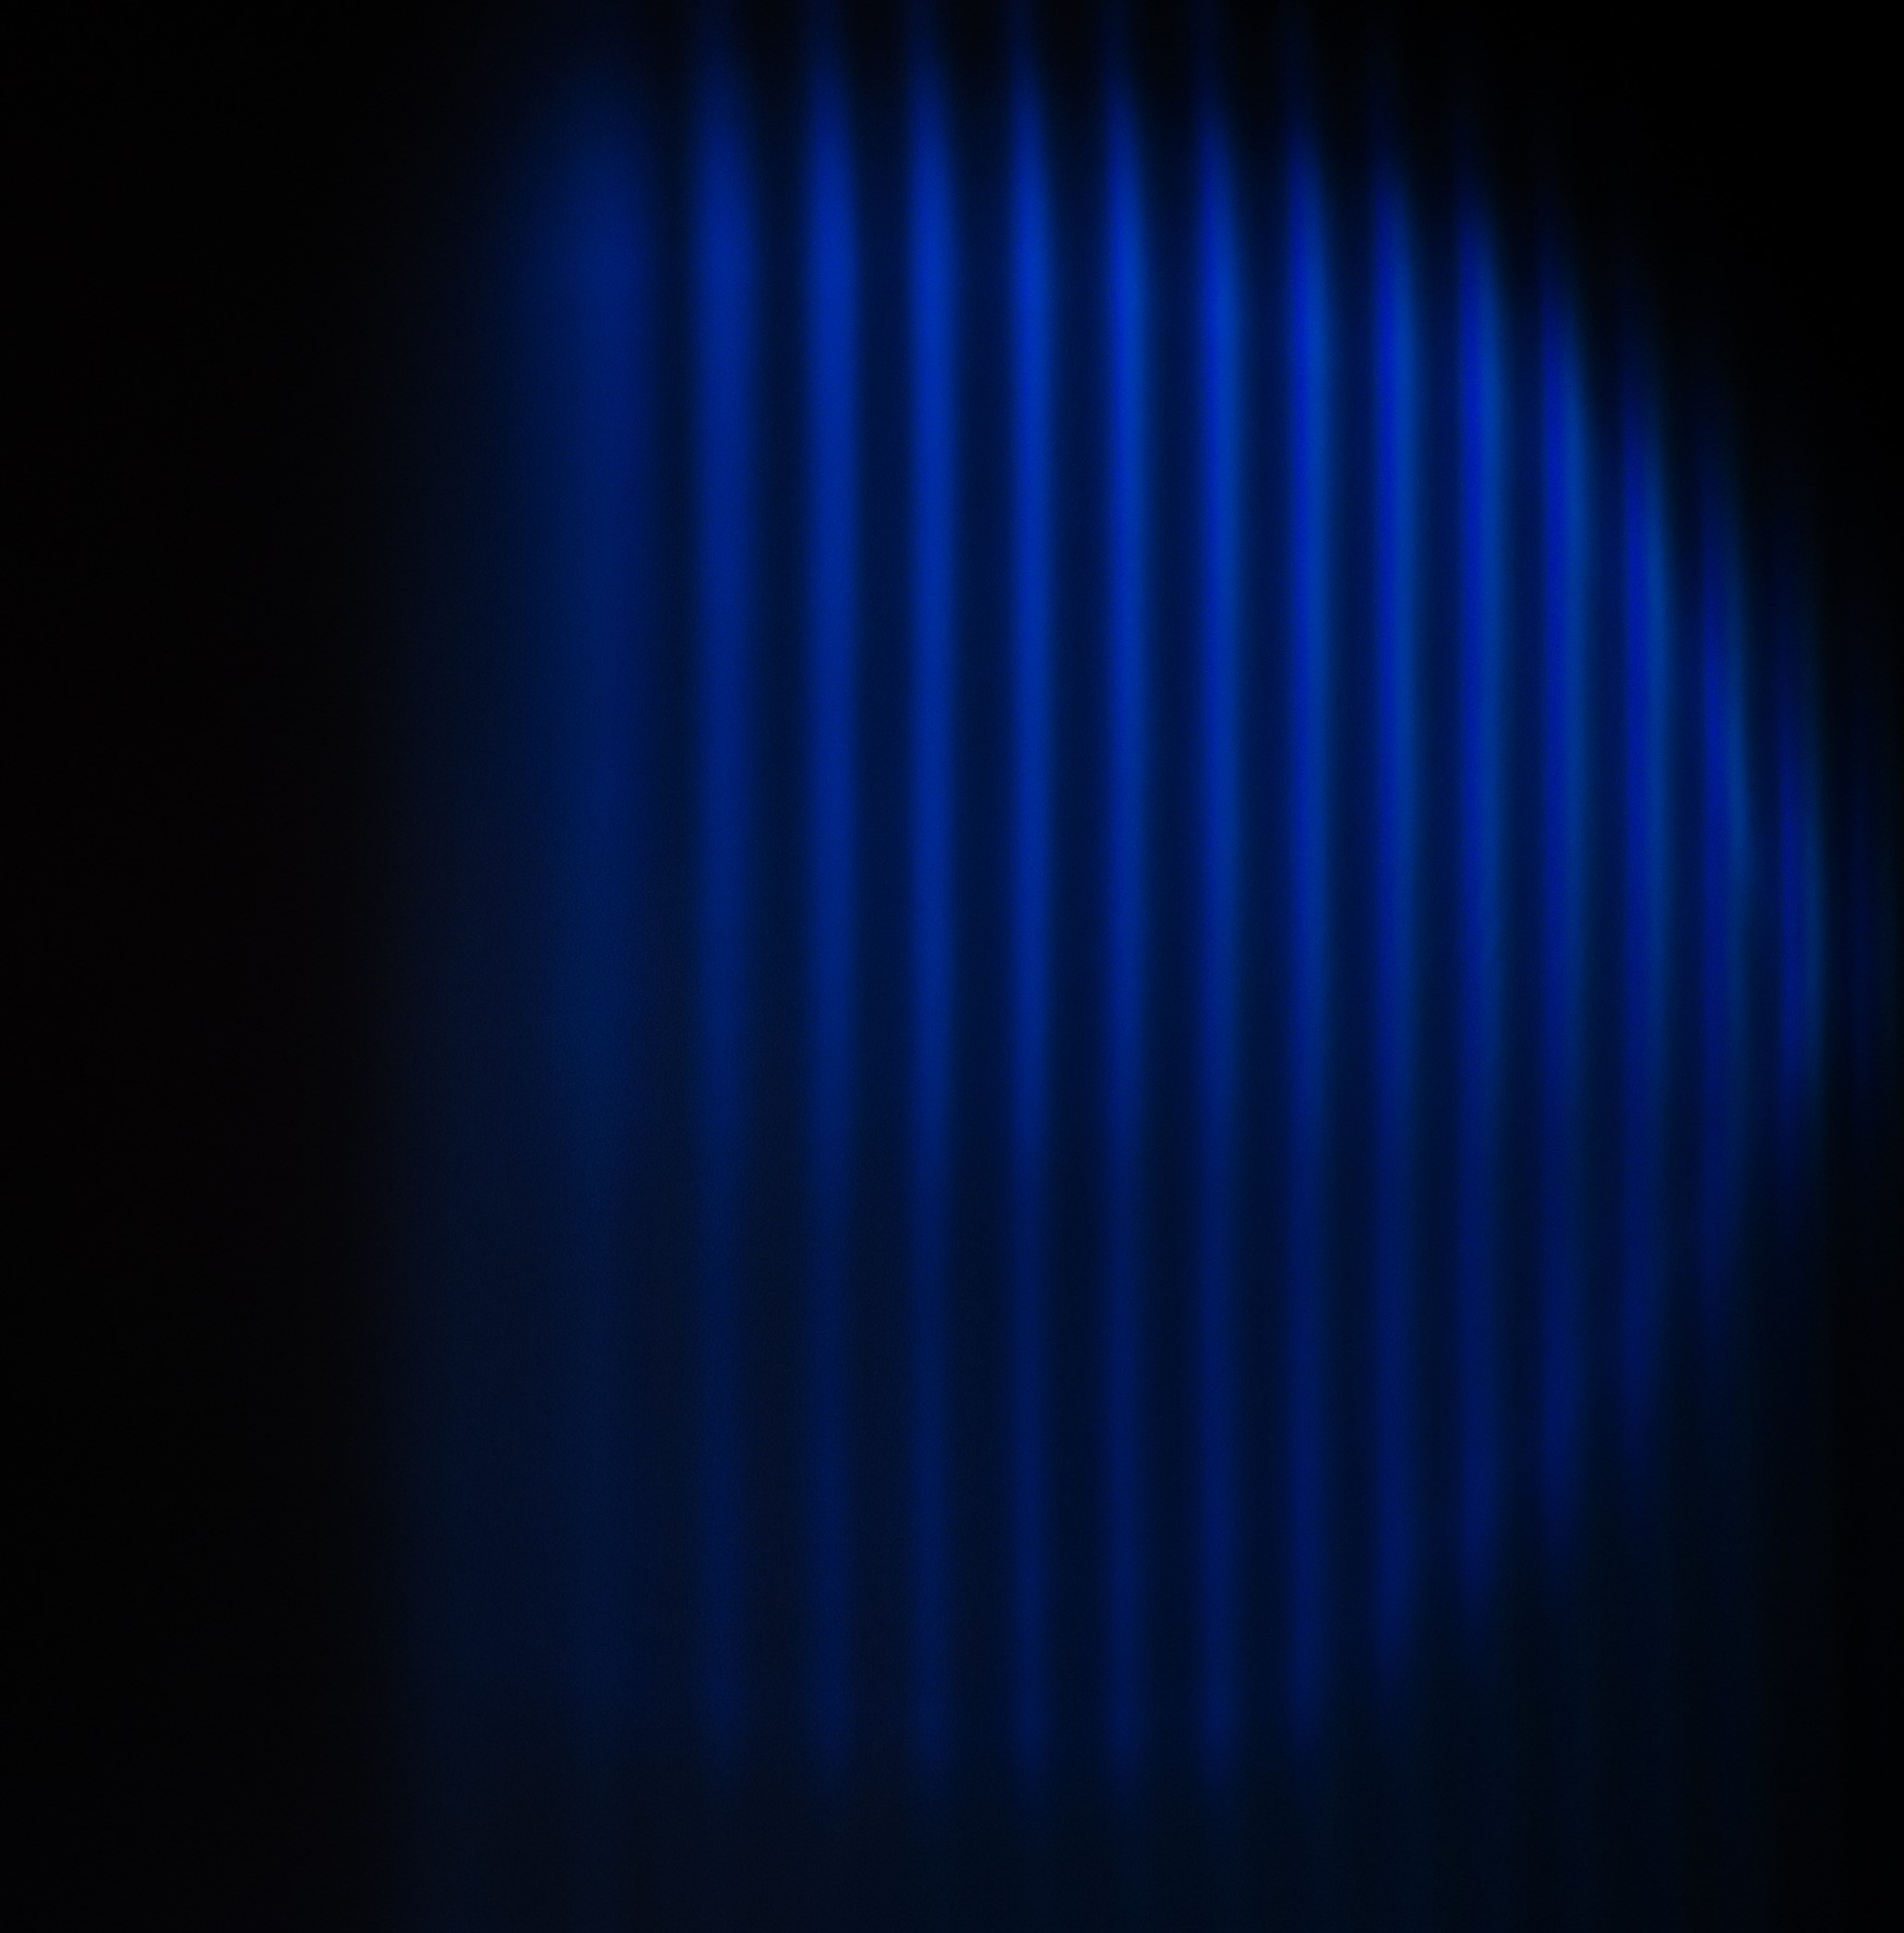
\includegraphics[width=0.5\textwidth]{bilder/3001_BLAU_0mT_pi.jpg}
  \caption{Fotographie der Interferenzlinien der Lummer-Gehrcke-Platte für die $\pi$-Linie des blauen Lichts ohne angelegtes Magnetfeld.}
  \label{abb:piblau0mT}
\end{figure}
\begin{figure}
  \centering
  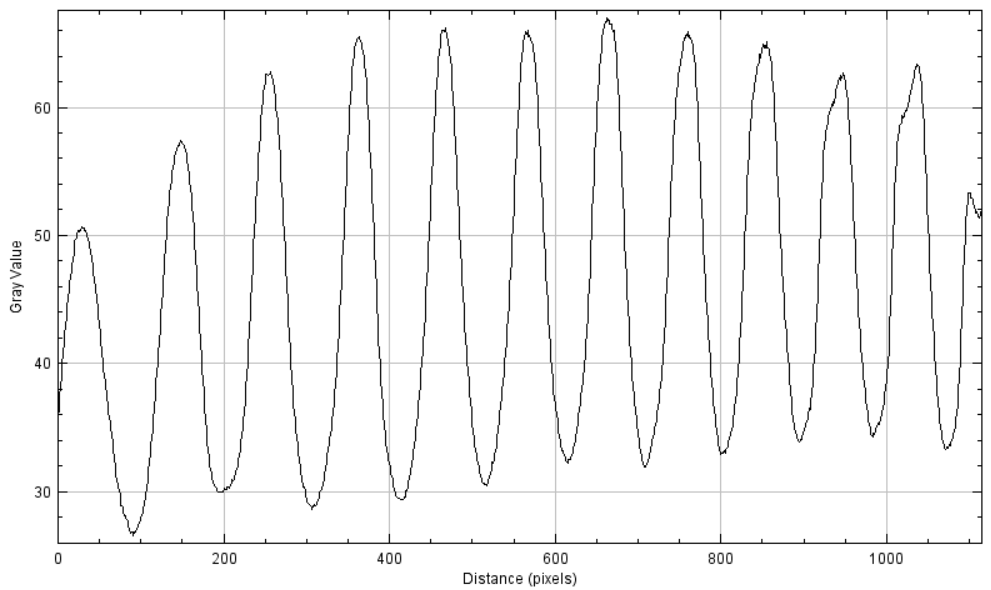
\includegraphics[width=0.7\textwidth]{bilder/pi_BLAU_0mT.PNG}
  \caption{Kontrastauswertung der Interferenzintensität für die $\pi$-Linie des blauen Lichts ohne ein angelegtes Magnetfeld. Aufgetragen ist die Intensität in beliebigen Einheiten gegen den Abstand in $x$-Richtung in Einheiten von Pixeln.}
  \label{abb:plotpiblau0mT}
\end{figure}
%--------------------------------------------------------------------------------
\begin{table}[H]
  \centering
  \caption{Mit dem Programm \textit{Fiji} \cite{Fiji} ausgelesene Intensitätsmaxima zur Bestimmung der Abstände $\deltaup s$ für die blaue Spektrallinie mit einem angelegten Magnetfeld $B=\SI{1060 \pm 50}{\milli\tesla}$ unter einem Polarisationswinkel von $90°$.}
  \label{tab:piblau1060mT}
  \begin{tabular}{c|cc}
    \toprule
    {Nummer} & {$x \:/\: \si{px}$} & {$y \:/\: \text{bel. Einheiten}$}\\
    \midrule
 1 &  101  &	 87,06 \\
 2 &  202  &	 94,00 \\
 3 &  296  &	 97,47 \\
 4 &  389  &	 99,59 \\
 5 &  478  &	 101,47 \\
 6 &  566  &	 101,63 \\
 7 &  651  &	 102,47 \\
 8 &  732  &	 101,96\\
 9 &  816  &   101,96 \\
10 &  895  &	 102,59 \\
11 &  972  &	 104,19 \\
12 &  1049 &	 103,60 \\
13 &  1122 &	 102,80 \\
14 &  1196 &	 102,14 \\
15 &  1267 &	 100,67 \\
  \end{tabular}
\end{table}

\begin{figure}
  \centering
  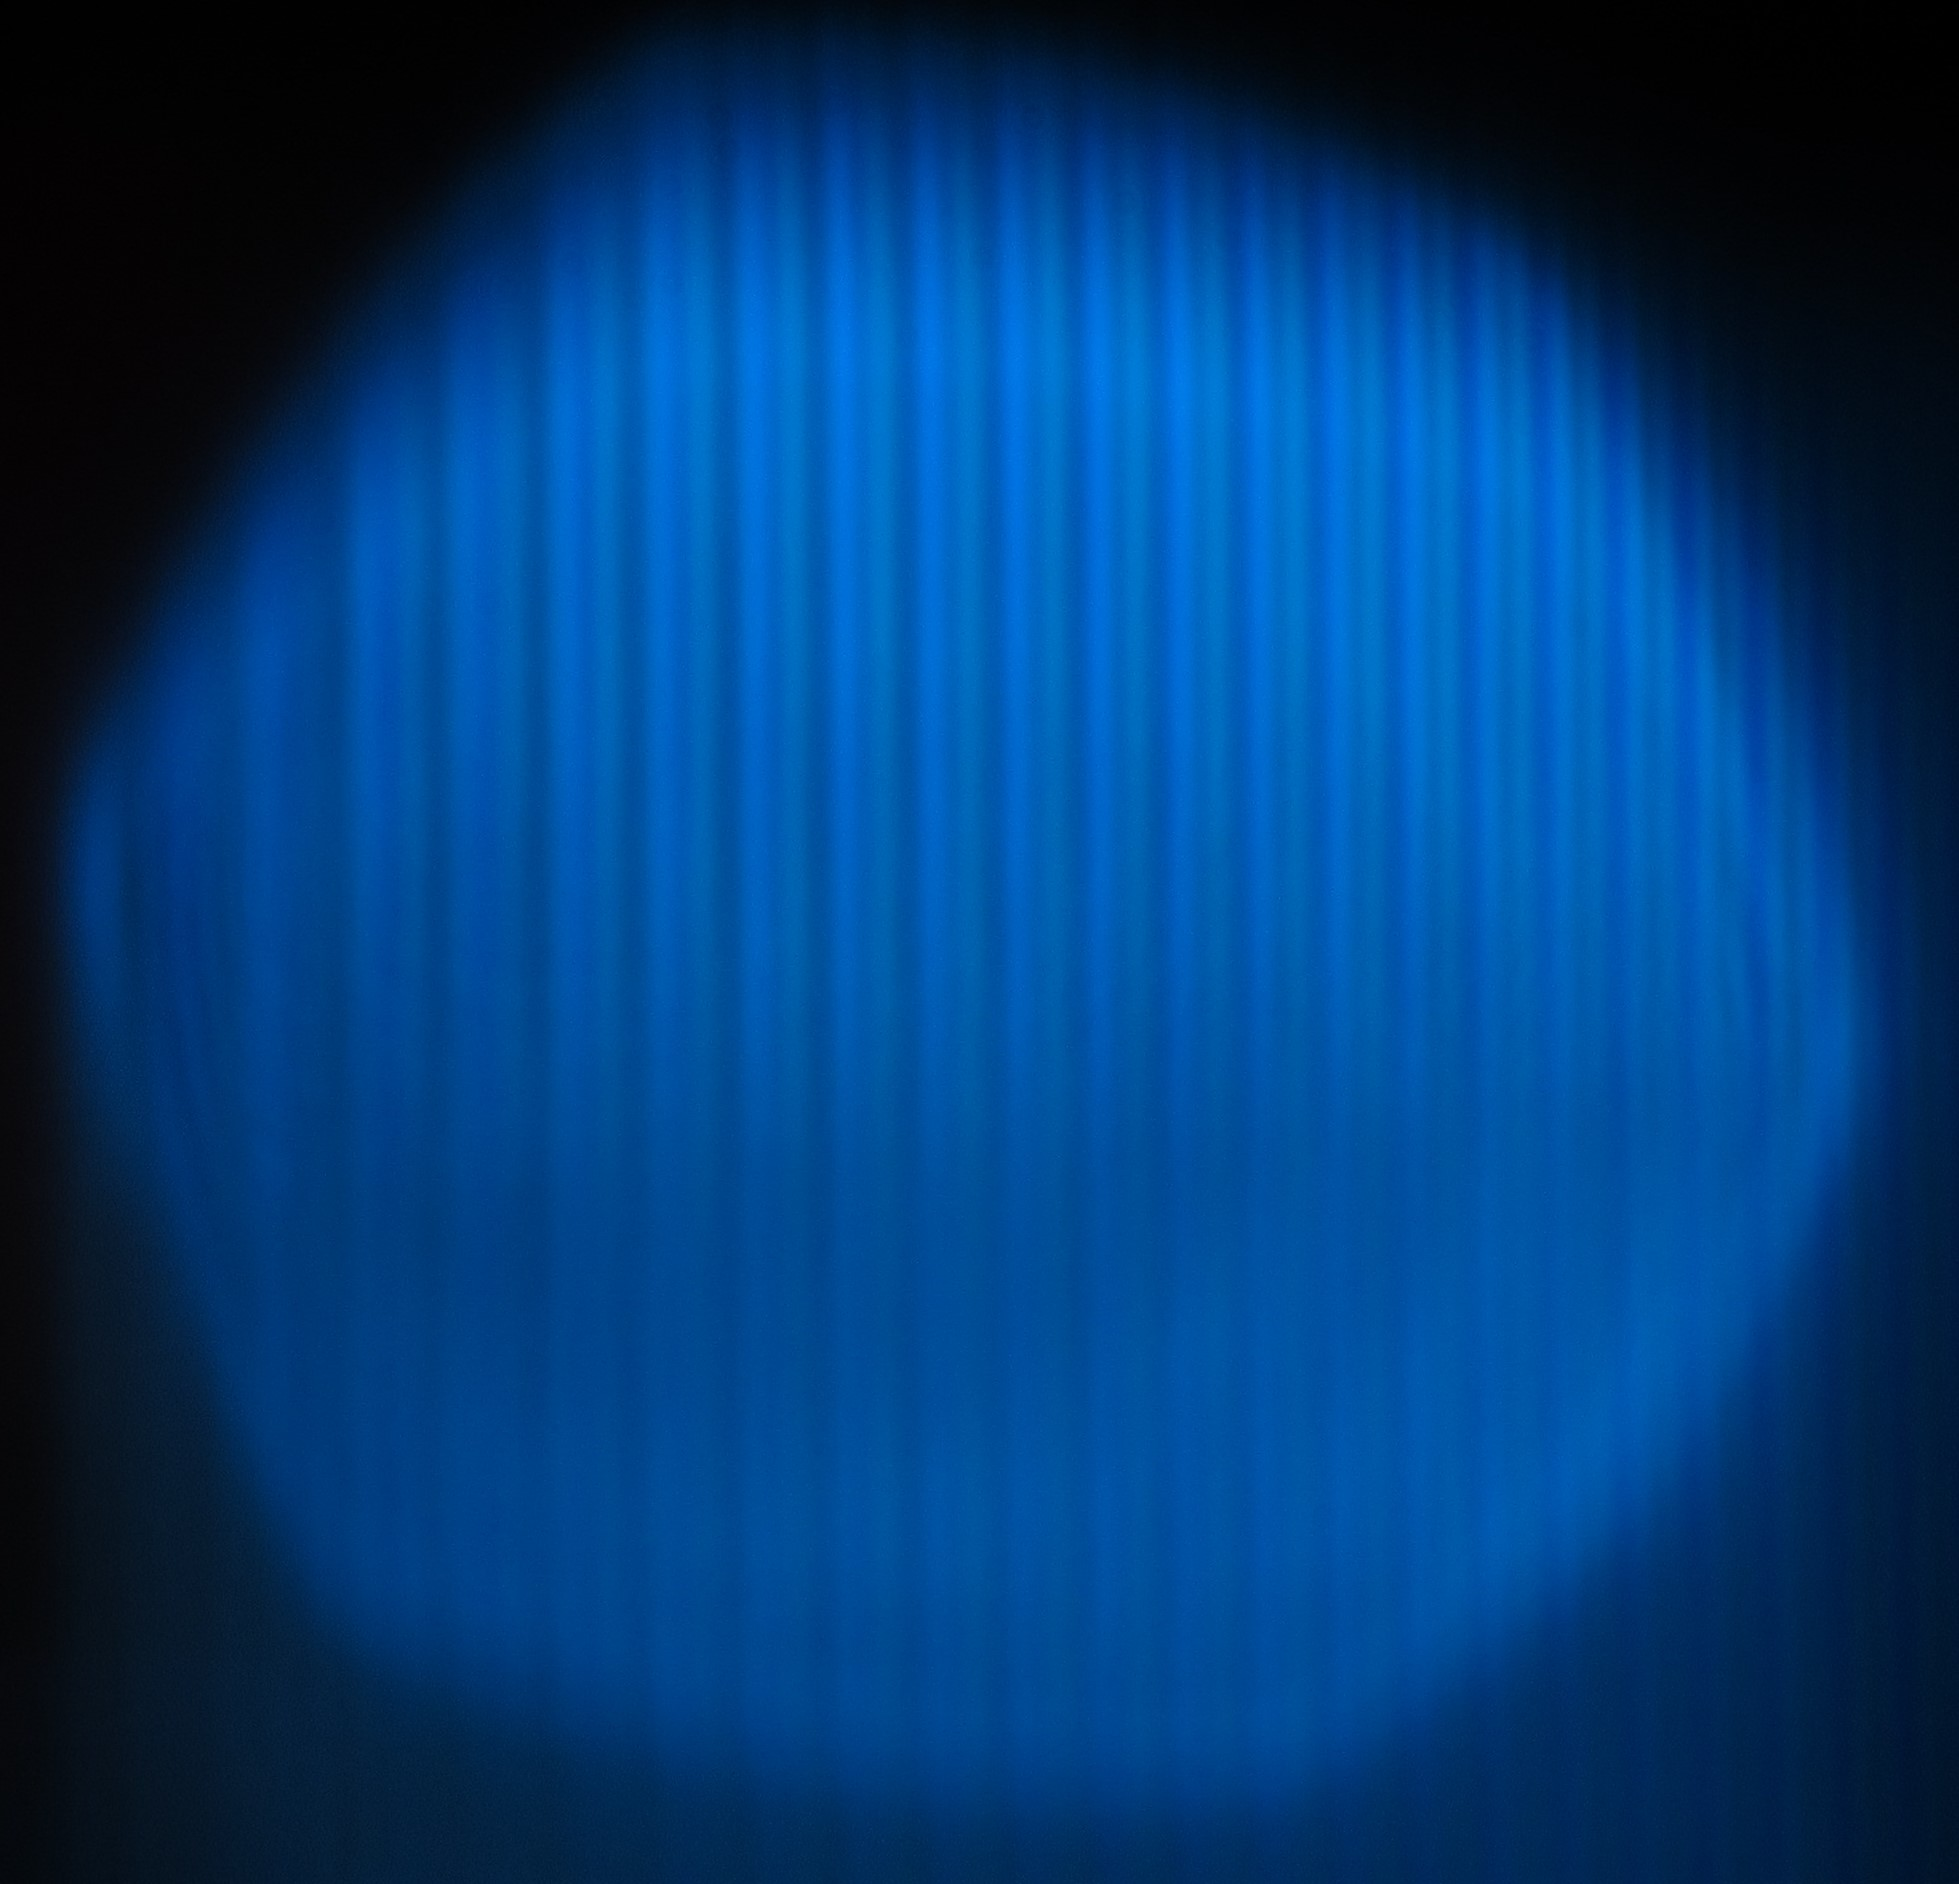
\includegraphics[width=0.5\textwidth]{bilder/3009_BLAU_1100mT_pi.jpg}
  \caption{Fotographie der Interferenzlinien der Lummer-Gehrcke-Platte für die $\pi$-Linie des blauen Lichts bei einem angelegten Magnetfeld von $B=\SI{1060 \pm 50}{\milli\tesla}$.}
  \label{abb:piblau1060mT}
\end{figure}
\begin{figure}
  \centering
  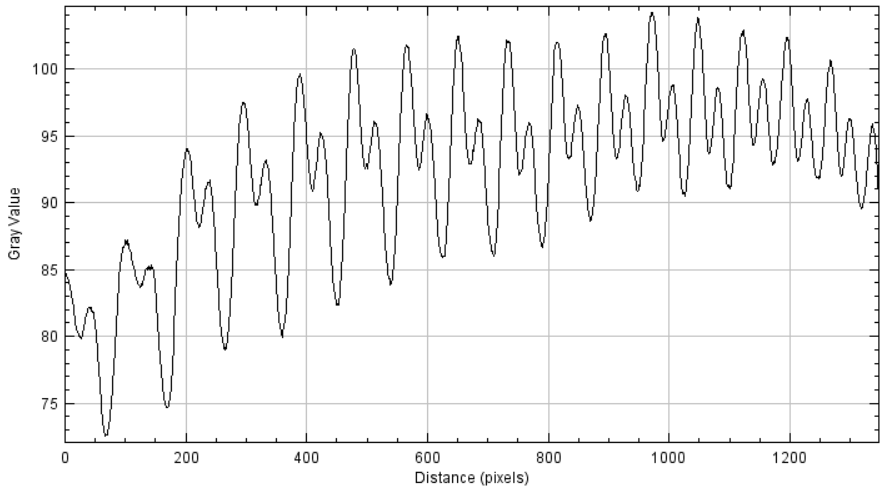
\includegraphics[width=0.7\textwidth]{bilder/pi_BLAU_1100mT.PNG}
  \caption{Kontrastauswertung der Interferenzintensität für die $\pi$-Linie des blauen Lichts bei einem angelegten Magnetfeld von $B=\SI{1060 \pm 50}{\milli\tesla}$. Aufgetragen ist die Intensität in beliebigen Einheiten gegen den Abstand in $x$-Richtung in Einheiten von Pixeln.}
  \label{abb:plotpiblau1060mT}
\end{figure}
